\subsubsection{Diagramas de flujo de datos:}

Refinamos el proceso de realizar gráfica en los cuatro requisitos funcionales junto al almacén de datos, que separamos en los almacenes Partidas y Estadísticas.
 
 
 \begin{figure}[h!]
 	\centering
 	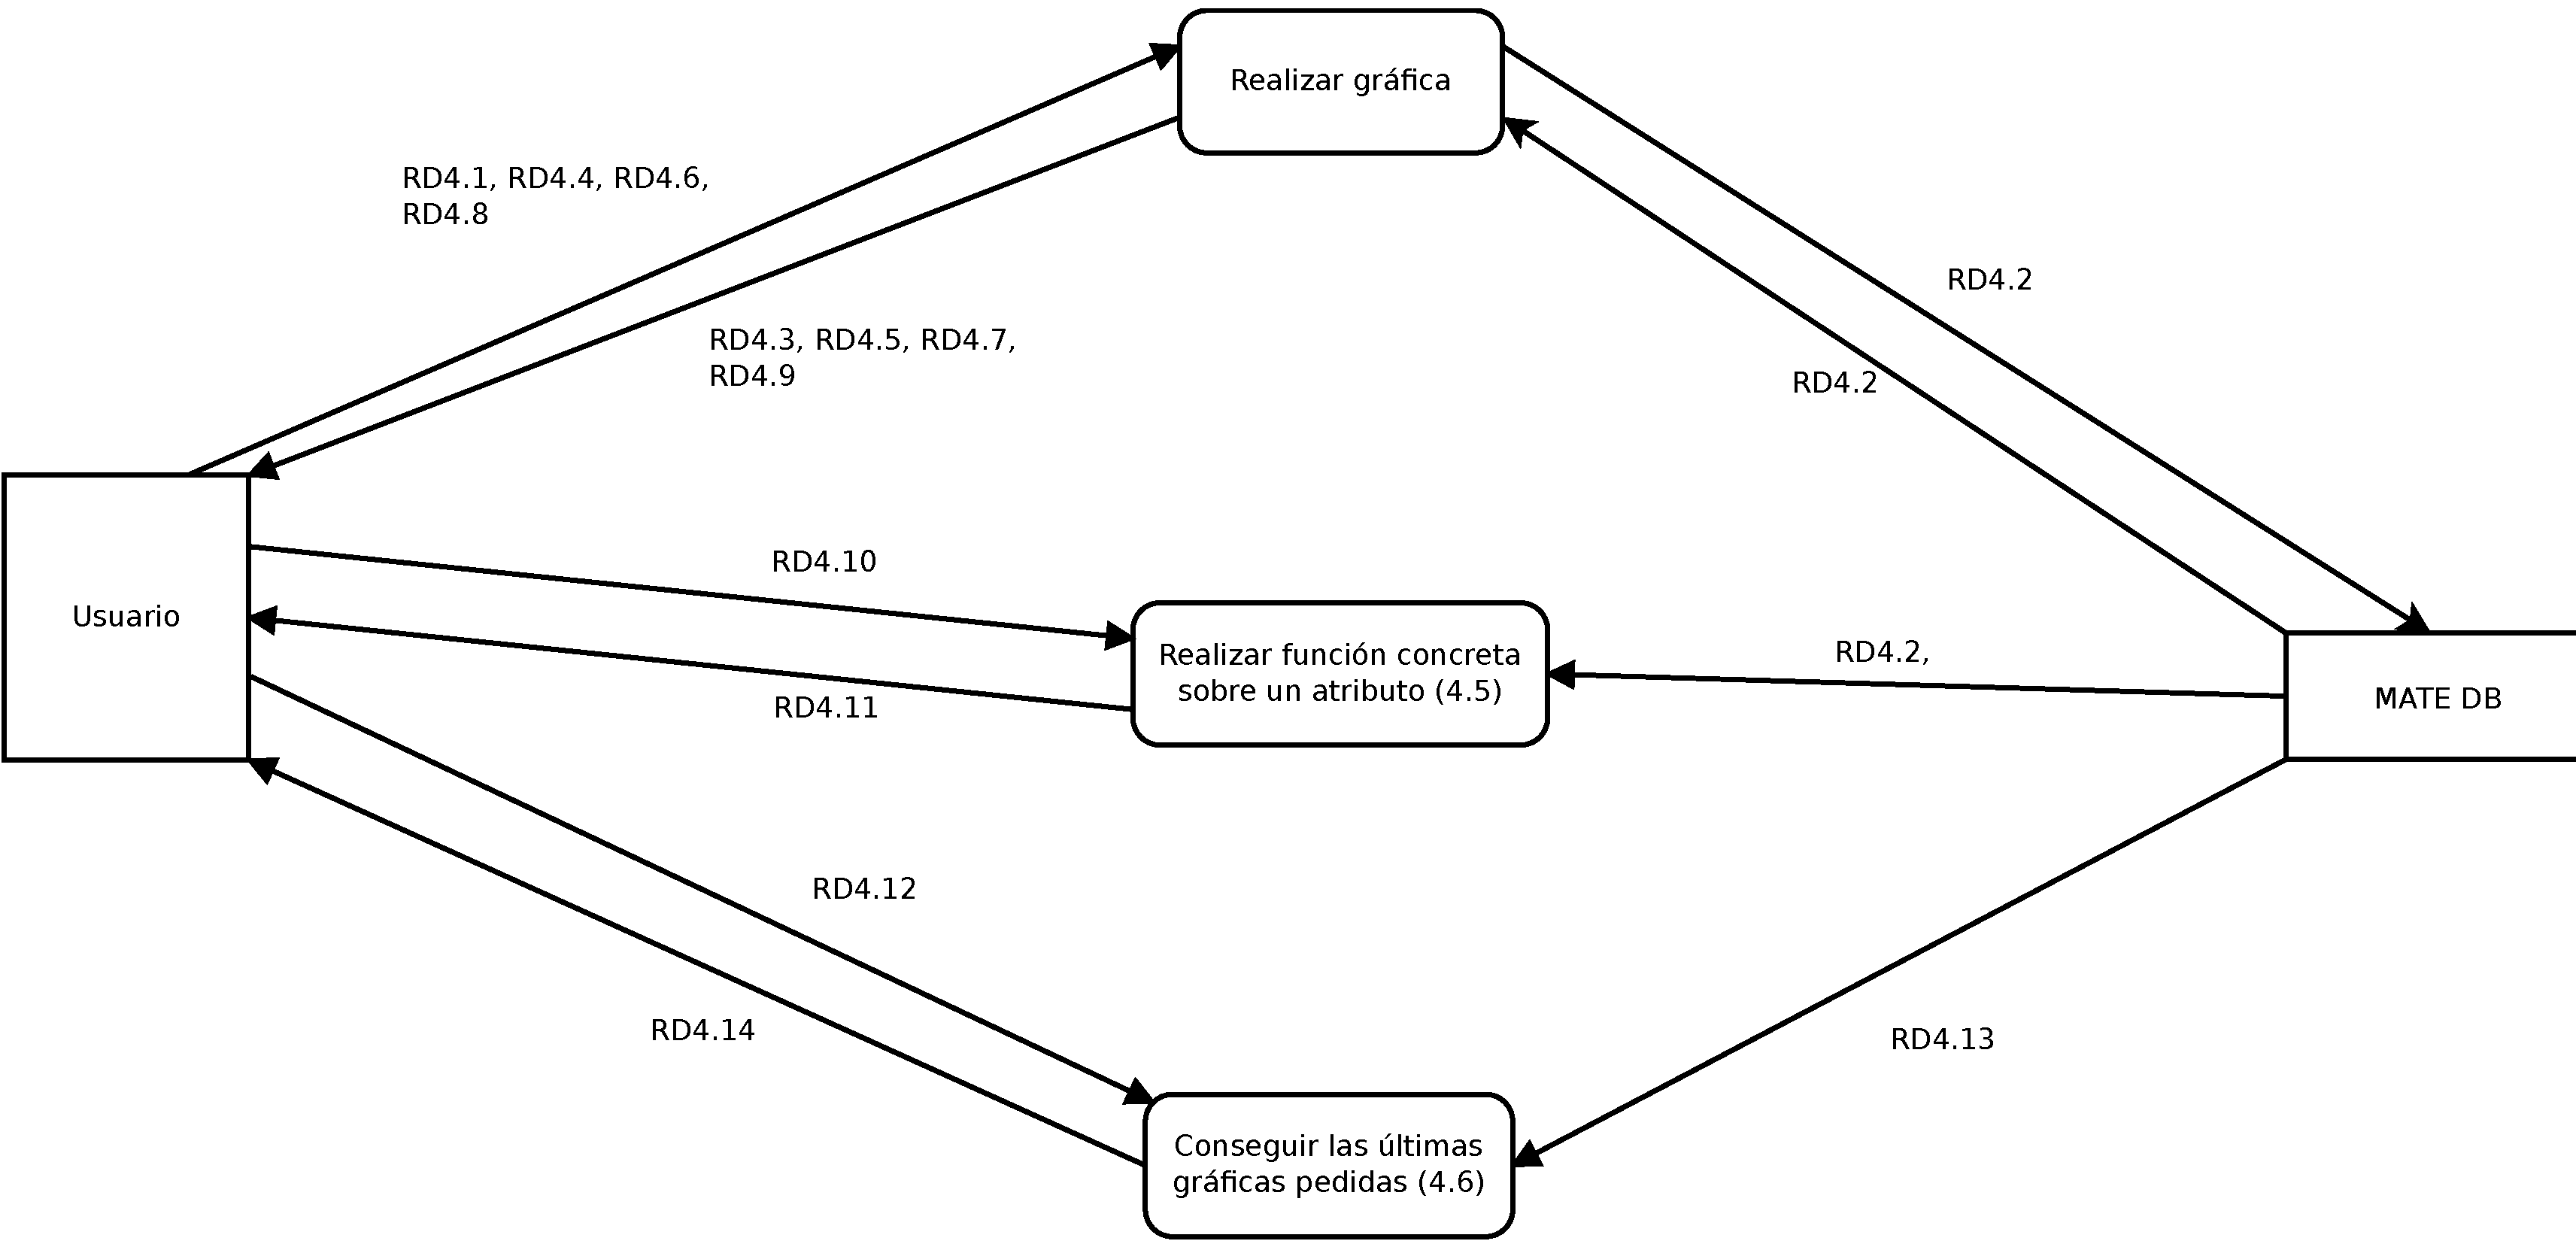
\includegraphics[width=0.7\linewidth]{../Diagramas/pdf/DiagramaEstadistica1.pdf}
 	\caption{Subsistema de estadísticas, nivel 1}
 	\label{fig:RefinamientoEstadisticas1}
 \end{figure}
 
 
 \begin{figure}[h!]
 	\centering
 	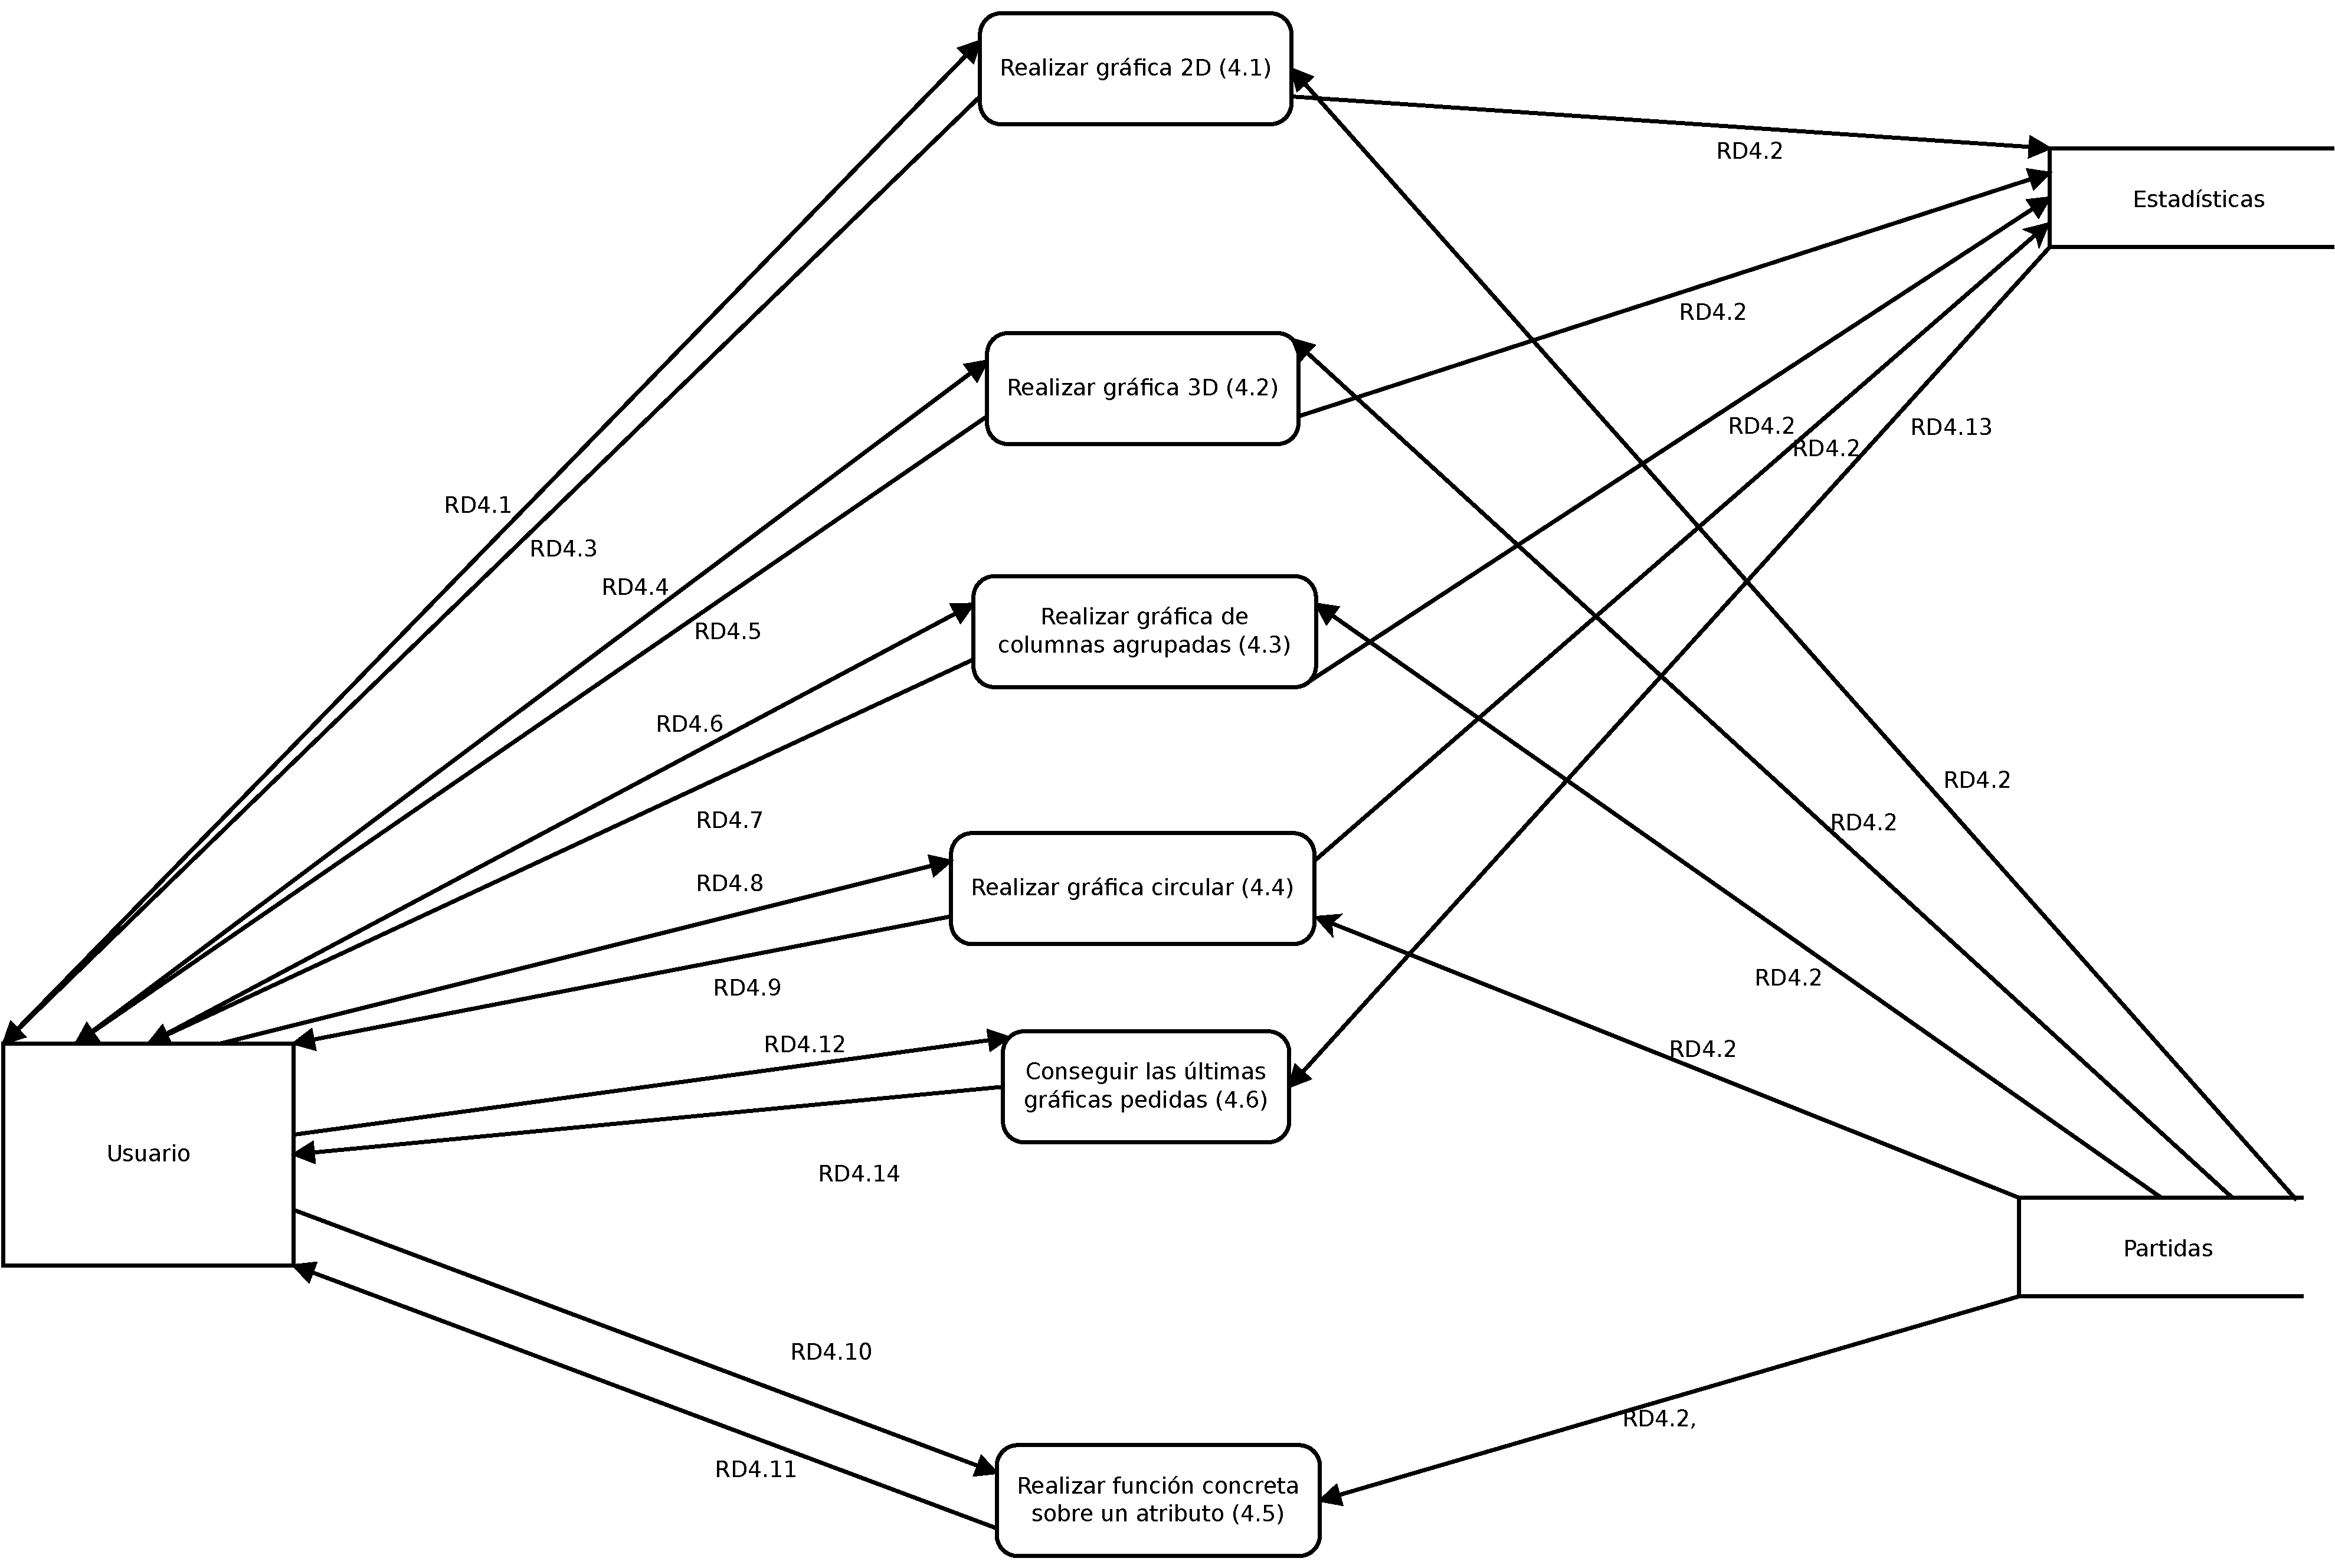
\includegraphics[width=0.7\linewidth]{../Diagramas/pdf/DiagramaEstadistica2.pdf}
 	\caption{Subsistema de estadísticas, nivel 2}
 	\label{fig:RefinamientoEstadisticas2}
 \end{figure}
 
 
\begin{figure}[H]
\centering
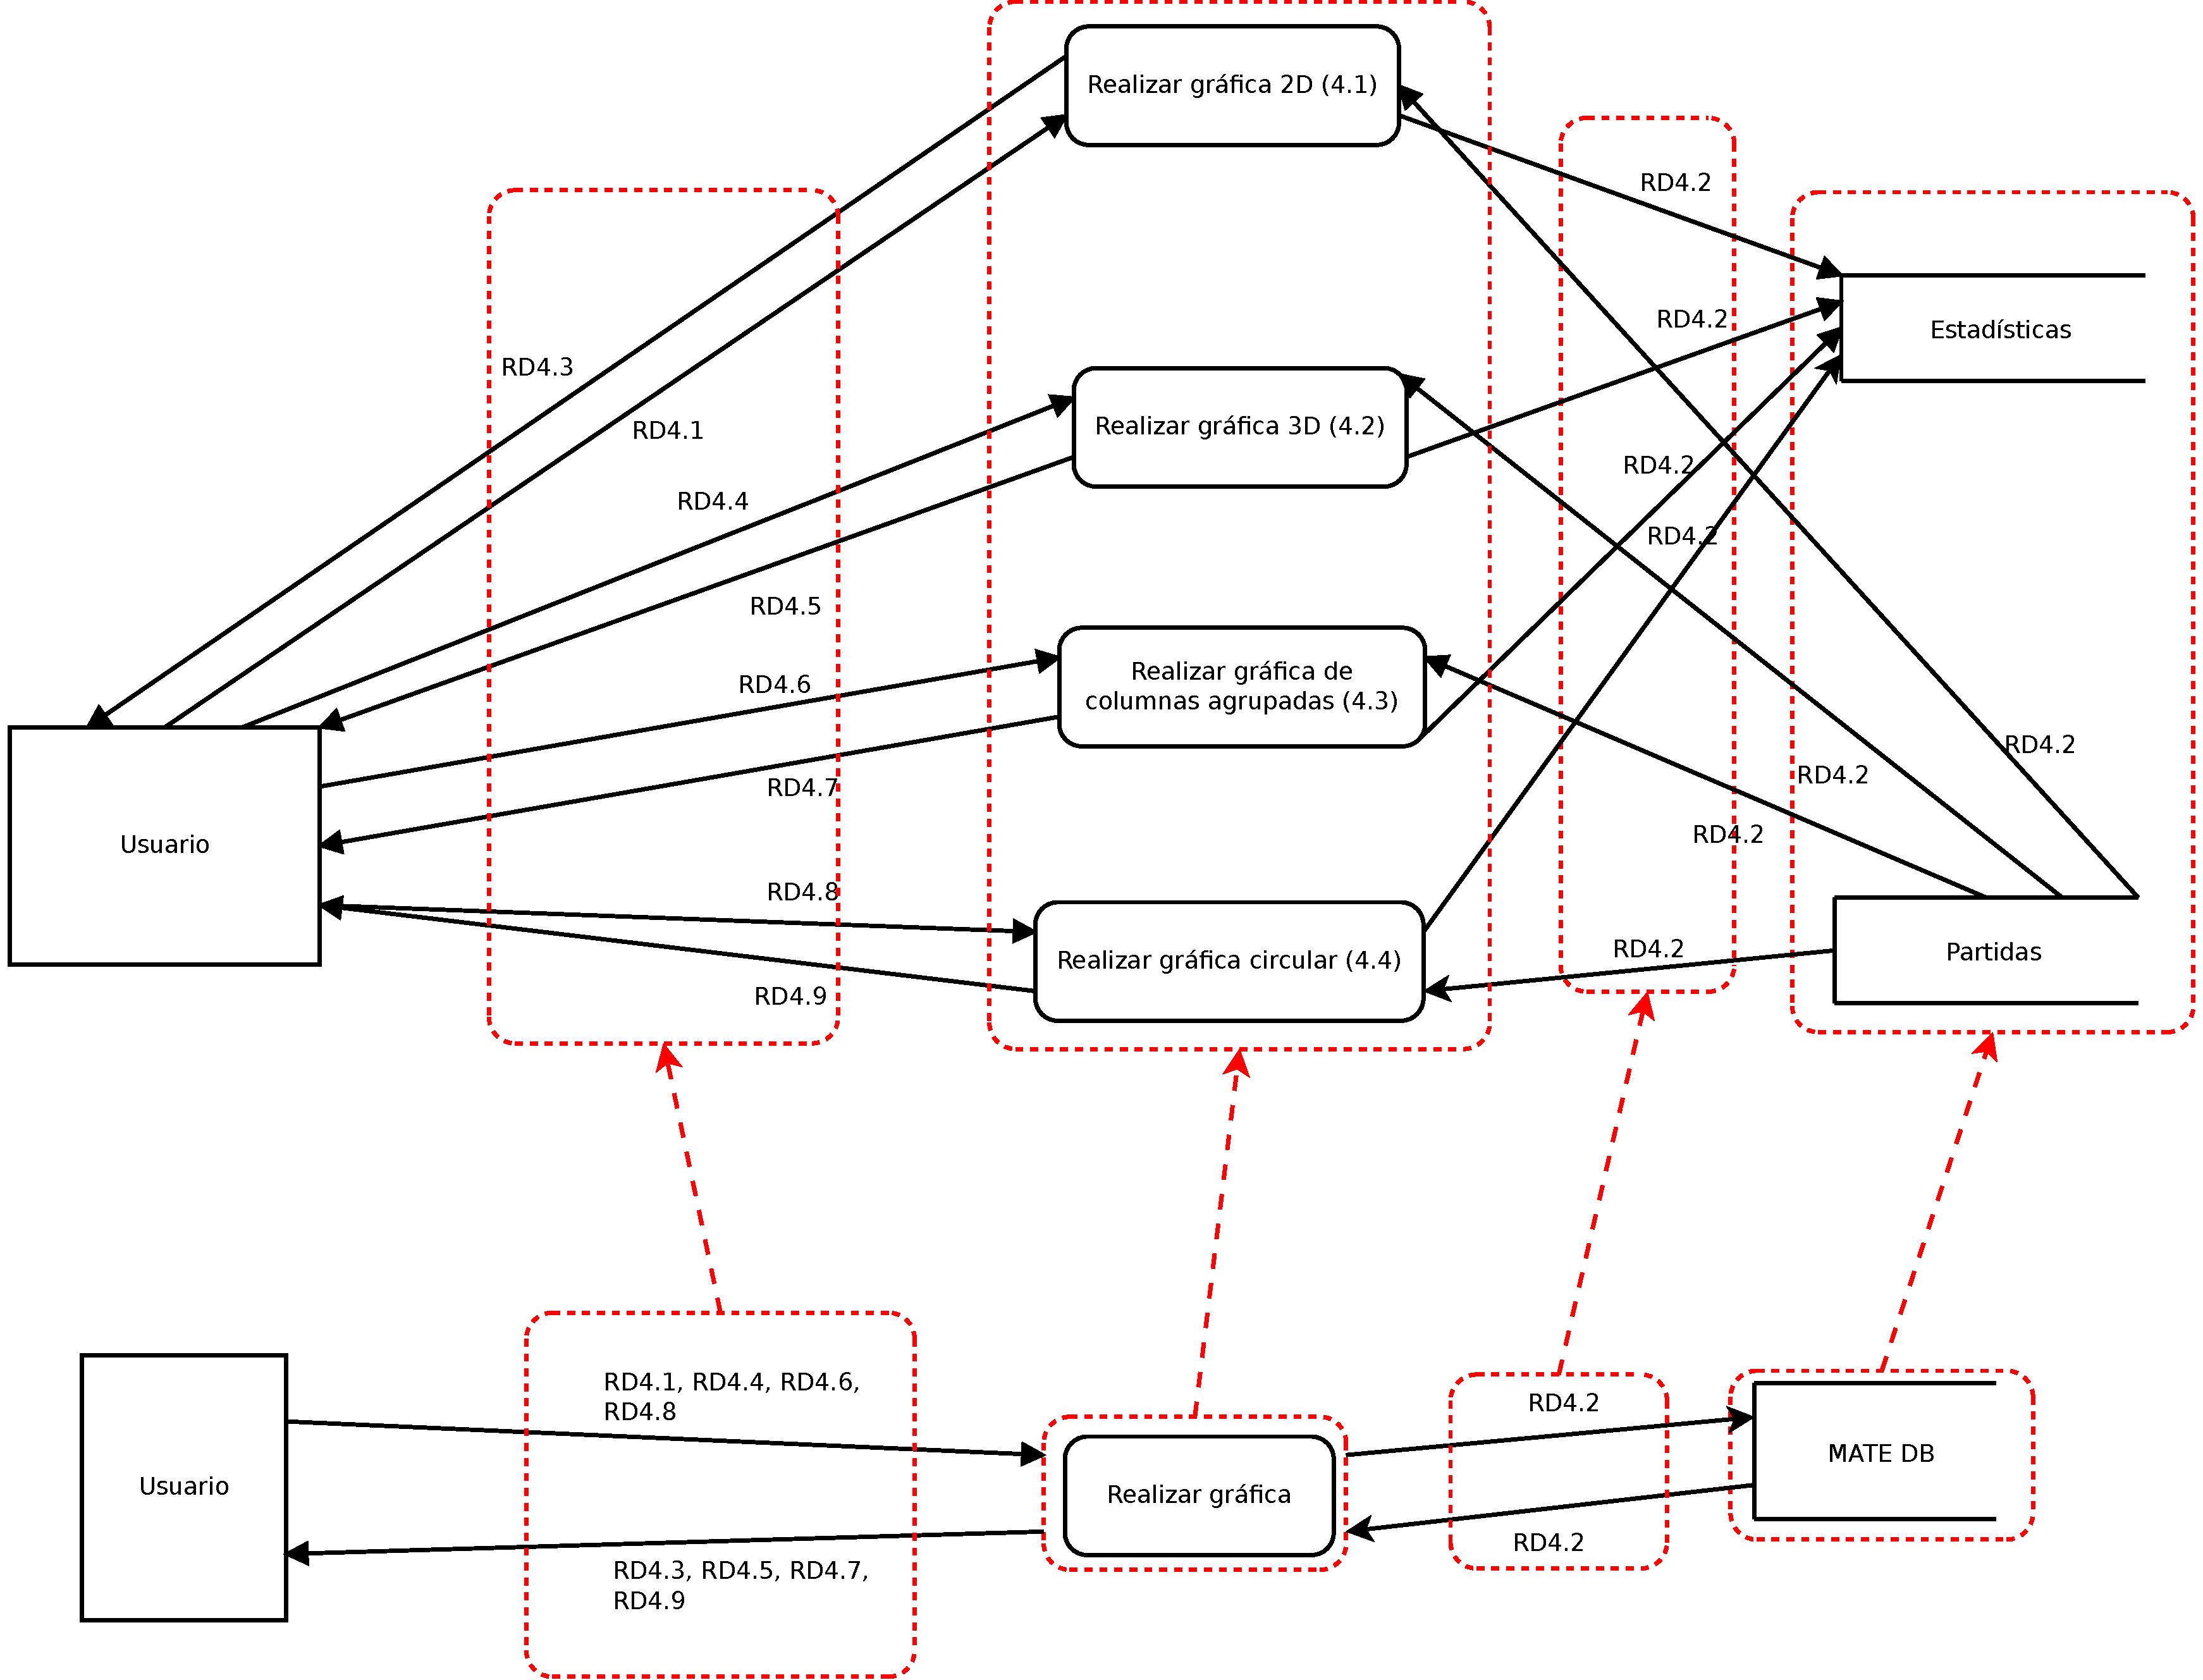
\includegraphics[width=0.7\linewidth]{../Diagramas/pdf/RefinamientoEstadisticas.pdf}
\caption{Refinamiento del diagrama de estadísticas}
\label{fig:RefinamientoEstadisticas}
\end{figure}


\newpage

\subsubsection{Diagramas externos y de entidad relación}

\begin{figure}[H]
	\centering
	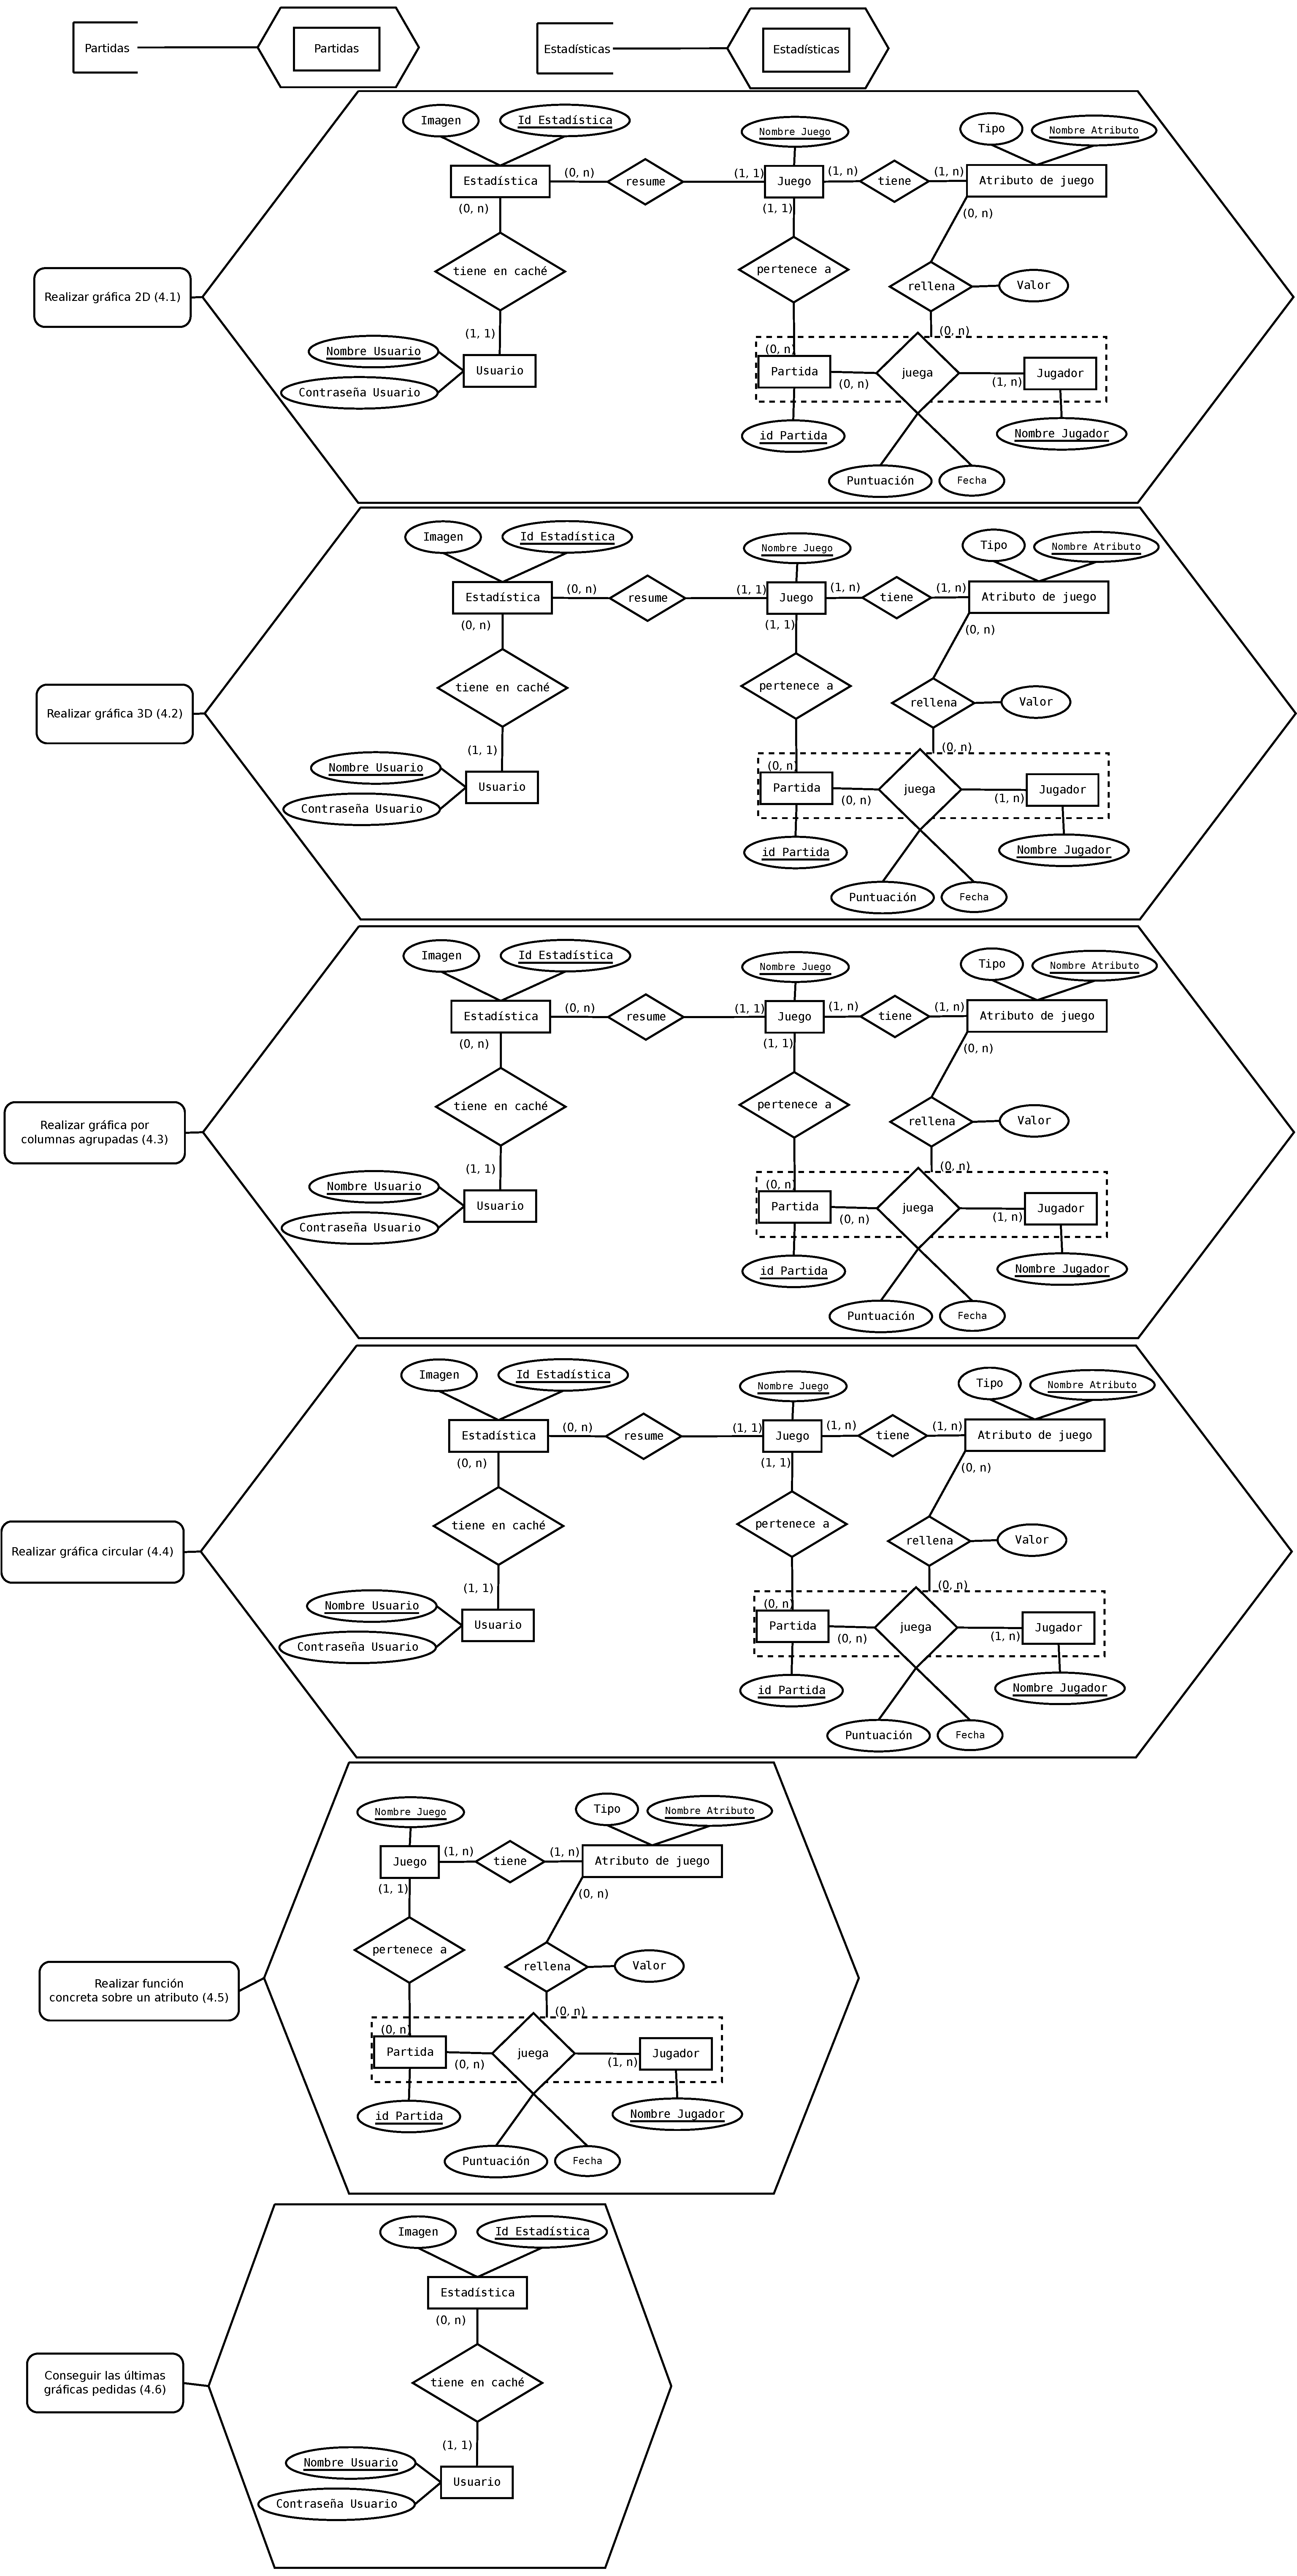
\includegraphics[width=0.6\linewidth]{../Diagramas/pdf/ExternoEstadisticas.pdf}
	\caption{Diagrama externo del susbsistema estadísticas}
	\label{fig:ExternoEstadisticas}
\end{figure}

\begin{figure}[H]
	\centering
	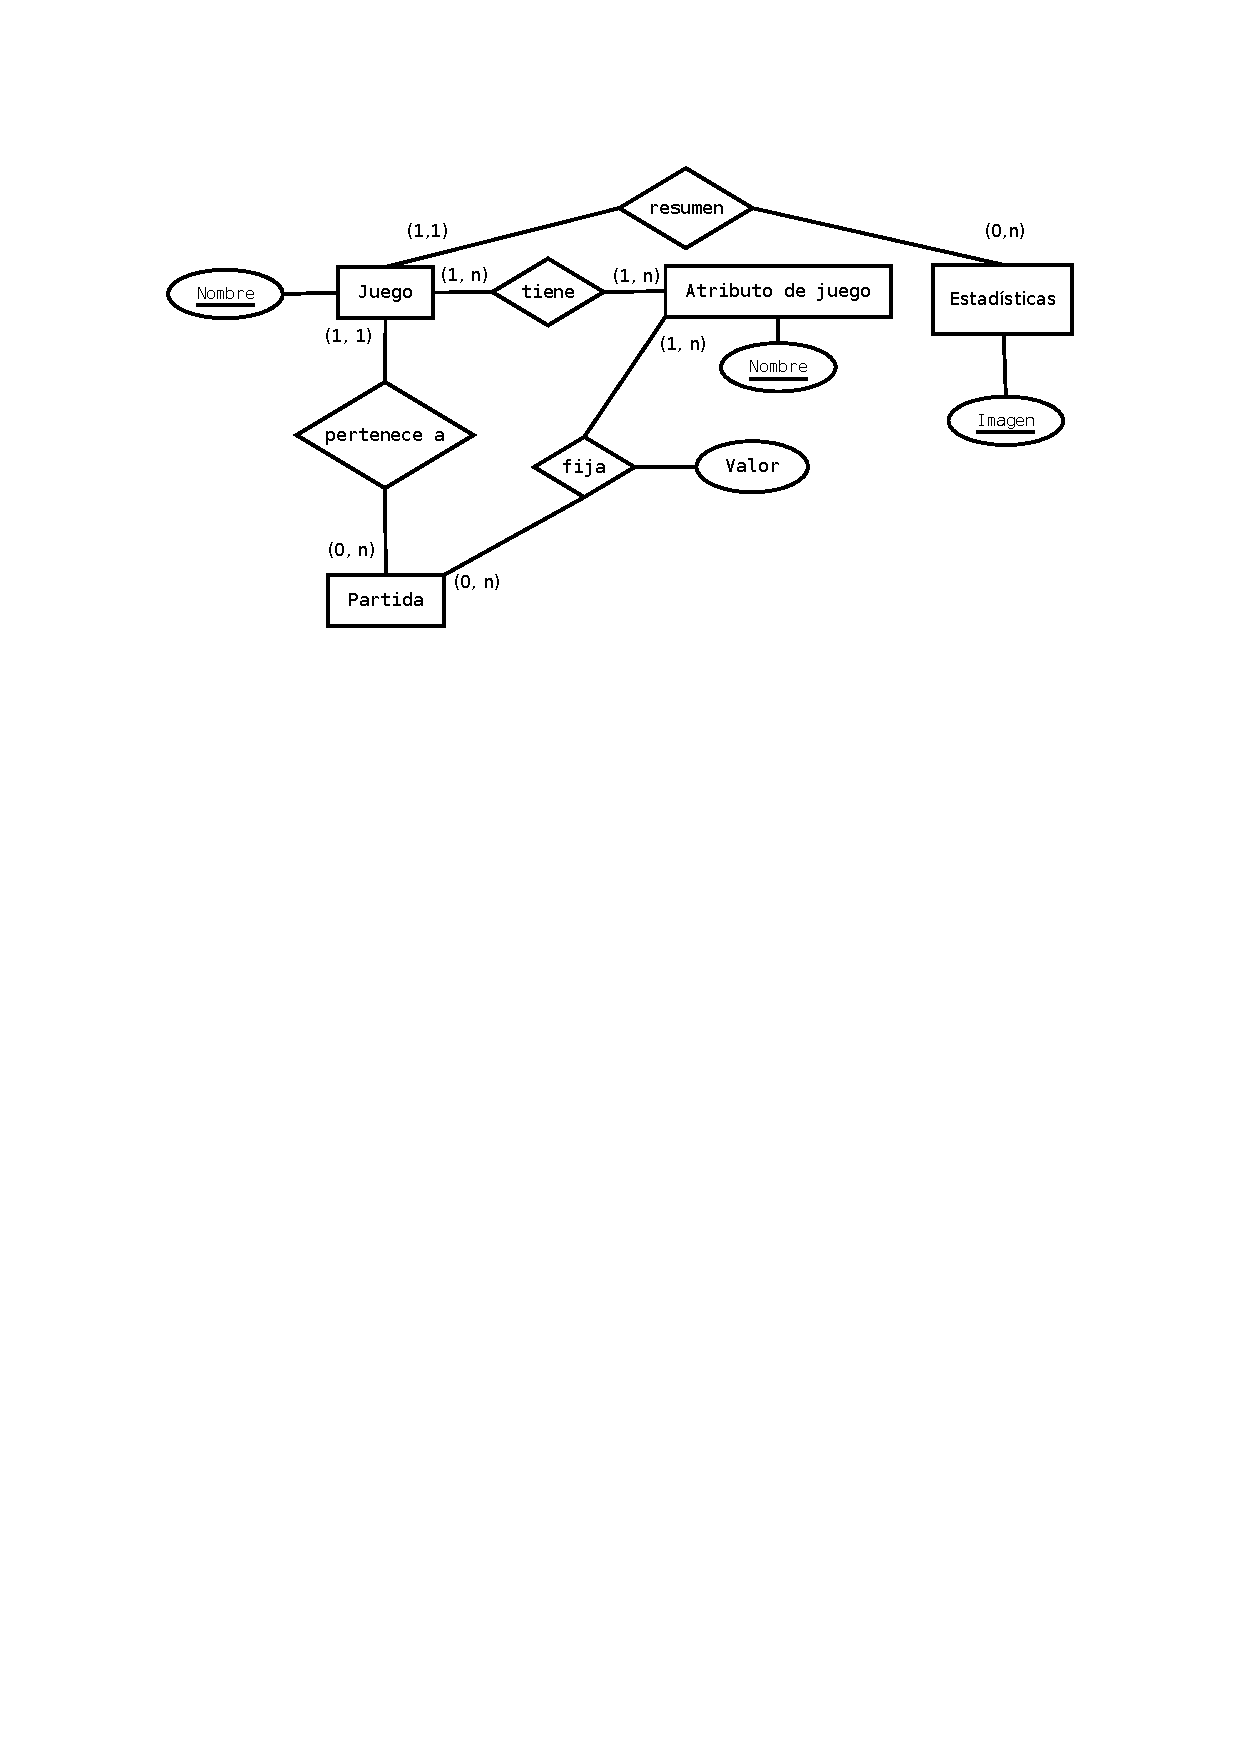
\includegraphics[width=0.7\linewidth]{../Diagramas/pdf/EREstadistica.pdf}
	\caption{Entidad relación del subsistema estadísticas}
	\label{fig:EntidadRelacion}
\end{figure}

\newpage